\chapter{Theoretische Grundlagen}
Das Projekt basiert auf einigen theoretische Grundlagen. Dazu zählen
neben neben Prinzipien und Lerntheorien einige technische Begriffe, deren
Erläuterungen Inhalt dieses Kapitels sind. Dabei handelt es sich großenteils um
eine Kurzfassung der Beschreibungen aus \cite{gruben:2012}.

\section{Prinzipien und Theorien}
\subsection{Lernen}
Das Lernen selbst wird heute als ein Prozess verstanden. Dabei wirken "`mehrere
zentrale psychologische Phänomene (Motivation, Emotion,
Kognition)"'\cite{niegemann:2004} zusammen. 

Der Lernprozess besteht dabei aus drei Abschnitten:
\begin{enumerate}
  \item Zunächst werden Eindrücke wahrgenommen. Dabei tragen neue oder
  vergessene Eindrücke zur Umstrukturierung im Gehirn bei.
  \item Umstrukturieren bedeutet, dass Synapsen bewegt und andere Gehirnzellen
  angekoppelt werden.
  \item Mit Wiederholungen wird Wissen persistiert. Es entstehen stabile
  Strukturen, welche einfach und schnell abrufbar sind.
\end{enumerate}
In Abbildung \ref{pic:structSyn} wird diese Umstrukturierung illustriert
\cite{spitzer:2012}.

Von ein LMS wird erwartet, dass es diesen Lernprozess unterstützt. Anfänger
sollen die Möglichkeit erhalten zunächst klein anzufangen und die Grundlagen
eines bestimmten Sachverhaltes kennenzulernen. Fortschreitend können die
Anforderungen und Herausforderungen gesteigert werden, um den Lernprozess zu
unterstützten und zugleich die Motivation aufrecht zu erhalten.

\begin{figure}[H]
\centering
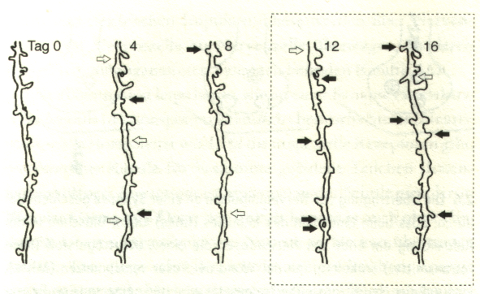
\includegraphics[width=0.7\textwidth]{SPIsynapseS50.png}
\caption{Umstrukturierung von Synapsen \footnotemark}\label{pic:structSyn}
\end{figure}\footnotetext{aus \cite{spitzer:2012}}

\subsection{Motivation}\label{ref:basMotivation}
Die Motivation ist ein wesentliches Standbein des Lernprozesses. Fehlt sie, so
ist es für Lernende bedeutend erschwert, Lerninhalte aufzunehmen, zu verarbeiten
und zu verstehen. Mithilfe von Motivation wird ein charakteristisches Verhalten
an den Tag gelegt, welches den Lernprozess aufrecht erhält \cite{jacobs:2010}.

Im Mittelpunkt jeder Motivation steht stets das persönliche Glück
\cite{stampfl:2012}. Dabei stehen Mittel zur Verfügung, die dem Lernenden auf
unterschliedliche weise unterstützen zu verstehen. Er kann zum einen
intrinsisch und zum anderen extrinsisch motiviert werden.

\subsubsection{Intrinsische Motivation}\label{ref:intrinsischeMotivation}
Die intrinsische Motivation wird auch als direkte Motivation bezeichnet. Damit
wird der Lernende direkt angesprochen und in seinen Bedürfnissen befriedigt und
seinen Wünschen wird unmittelbar nachgegangen. Ein intrinsisch motivierter
Lernender geht einer Tätigkeit im eigenen Interesse nach, es sind keine externen
Einflüsse nötig, die ihn zu seinen Handlungen erst bewegen müssen
\cite{jacobs:2010}.

Jede Lernsoftware hat aus dem zuvor erwähnten Sachverhalt die intrinsiche
Motivation zum Ziel. Dazu werden nicht selten unter Anderem auch gamifizierende
Inhalte verwendet (siehe \ref{ref:gamification}).

\subsubsection{Extrinsische Motivation}\label{ref:extrinsischeMotivation}
Die andere Seite der Motivation kommt von aussen. Es werden Belohnungen gegeben
oder Strafe und negative Konsequenzen vermieden. Synonyme sind demnach
"`indirekte Motivation"', das "`Butterbrot-und-Peitsche-Prinzip"' oder
"`Manipulation"' \cite{jacobs:2010}.

Für Masterly Mate im Speziellen, kann der Tutor ein extrinsisch Motivierender
Faktor sein. Hinzu kommen die gamifizierenden Elemente der zu erreichenden
Punktzahl pro WBT und das Aufsteigen in Rängen. Implizit wird auch Strafe in der
Form angewandt, dass es laut Konzept auch möglich ist, im Rang zu fallen
(siehe dazu Tabelle \ref{tab:privilegesRoles}).

\subsection{Lernmodelle}
Zum Zweck der Unterstützung des Lernprozesses und Förderung der Motivation haben
sich einige Lernmodelle herauskristallisiert, die heute als gültig und
vertretbar angesehen werden. In der Idee von Masterly Mate sind explizit zwei
Lernmodelle verwoben. Das Dreyfus fünf Etappen Modell mentaler Aktivitäten und
Blended Learning.

\subsubsection{Das Dreyfus fünf Etappen Modell mentaler
Aktivitäten}\label{ref:dreyfus}
Inhalt des Dreyfus-Modells ist das Hinterfragen, welche Person einer anderen
einen bestimmten Sachverhalt erklären sollte. Dabei wird insbesondere
berücksichtigt, wie groß der Unterschied der Fachkompetenz zwischen Lernenden
und Lehrenden ist. Es wurden insgesamt fünf Ränge\footnote{Novice, Competence,
Proficiency, Expertise, Mastery} definiert, die den Lernweg von abstrakten
Prinzipien hin zu konkreter Erfahrung mit der Aneignung von Wissen beschreiben
\cite{dreyfus:1980}.

Allgemein formuliert sollte kein Experte einem Neuling etwas erklären. Steigt
man neu in ein Fachgebiet ein, so sind zunächst simple und einfache Beispiele
verbunden mit einem engen Betrachtungswinkel des Sachverhalts sehr hilfreich.
Ein Experte würde den Neuling mit unnötigen Details überhäufen.

Dazu staffelt sich der Lernerfolg in fünf Etappen:
\begin{description}
  \item[1. Novize] Ein Novize ist auf grundlegende Anweisungen angewiesen. Er
  verfügt über kein Vorwissen und evaluiert sich nicht selbst. Mit extrinsischem
  Feedback wird dem Abkommen vom Regelwerk zuvorgekommen.
  \item[2. Fortgeschrittener] Die Handlungen des Fortgeschrittene sind gegenüber
  dem Novizen weniger kontextfrei. Sein weiterer Lernweg kann auf seiner kleinen
  Wissensbasis aufbauen. Er hat grundlegende Prinzipien verstanden und erkennt
  situationsbasierte Muster. Der Fortgeschrittene kann simple Beispiele anhand
  von Guidelines durchlaufen, er experimentiert jedoch nicht.
  \item[3. Erfahrener] Der Umgang mit typischen Situationen am ihm gegebenen
  System stellen keine Hürden für den Erfahrenen dar. Ihm ist es möglich neue
  Situationen anzuknüpfen, einzuordnen und sehr ähnliche bewusst zu
  unterscheiden. Der Erfahrene arbeitet nach selbst erschaffenen Maximen.
  \item[4. Experte] Der Experte ist kein geeigneter Lehrer für einen Novizen
  mehr. Er hat die grundlegenden Prinzipien verloren und arbeitet nach seiner
  Intuition, einer Mischung aus Regeln, Guidelines und Maximen. Lösungen für
  ungewohnte Situationen gehören stets zum Reportoir des Experten. Im Sinne der
  fachlichen Kompetenz ist dieser Grad der höchste.
  \item[5. Meister] Ein Meister zeichnet sich gegenüber dem Experten neben
  fachlicher Kompetenz durch herausragende didaktische Fähigkeiten aus. Er
  bleibt damit auch ein geeigneter Lehrer für Novizen.
\end{description}

Generell sollte sich ein Lehrer zwei Grade über seinem Schüler befinden oder
Meister sein. Weitere detailliertere Erklärungen zu den Rängen finden sich in
\cite{gruben:2012}.

\subsubsection{Blended Learning}\label{ref:blendedLearning}
Zweck des Blended Learning, zu deutsch auch Integriertes Lernen genannt, ist das
Verschmelzen der Vorteile diverser Lernformen. Darunter befinden sich
\ac{F2F}-Education, \ac{DE} und \ac{OE} (eLearning). Die jeweiligen Nachteile
wurden dabei weitestgehend überwunden \cite{kroeger:2004}.

Masterly Mate verfolgt die Verschmelzung von F2F-Education, der Durchführung von
Präsenzunterricht, mit eLearing, dem Durcharbeiten von WBTs. Die DE wird dabei
nur am Rande betrachtet, da nur in Ausnahmefällen Unterweisungen über Chats oder
ähnliche Kommunikationskanäle vonstatten gehen sollen.

\subsection{eLearning}
Mit dem eLearning wird im Gegensatz zum regulären Lernprozess ein zusätzlicher
Mittler, eine elektronische Komponente, zwischen die rohen Informationen und dem
lernenden Individuum eingeschoben. Heute ist beispielsweise ein Webbrowser ein
Wiedergabemedium von Vielen, welches der Demonstration von Informationen dient
\cite{baumgartner:2002}.

\subsubsection{Vorteile}
ELearing ist grundsätzlich unabhänig von physischen Gegebenheiten, mithilfe von
Software lassen sich sämtliche, auch fiktive, Szenarien darstellen. Der
Kreativität sind keine Grenzen gesetzt. Auch ist eine enorm vereinfachte
Auswertung von Prüfungen und Tests möglich, da Computer zur Automatisierung von
Prozessen geschaffen sind. 

Für Masterly Mate bedeutet das, dass das Aufsteigen in höhere Ränge
automatisiert vonstatten gehen kann. Beim Überschreiten bestimmter Schwellwerte für Punkte
steigt der Lernende wie von selbst einen Rang auf. Es wird zudem möglich,
Statistiken für den Nutzer anzufertigen, was das Prinzip des gamifizierens
(siehe Abschnitt \ref{ref:gamification}) zusätzlich unterstützt. Das
Masterly Mate selbst ein digitales Produkt ist, spielt darüber hinaus der
eigenen vereinfachten Verbreitung über nationale Grenzen hinweg stark zu.

\subsubsection{Nachteile}  
Grundsätzlich ist der Unterschied zwischen Mensch und Maschine der größte
Gegner von eLearning. Ein Computer kann heute nur recht spärlich auf die
Bedürfnisse des Lernenden eingehen. 

Expertensystemen wird beispielsweise nur eine beratende Funktion zugeteilt.
Weitere Beispiele sind neuronale Netze, welche zwar Lösungen entwickeln können,
jedoch muss deren Erarbeitung überwacht und hinterfragt werden
\cite{keller:2000}.

Letztlich kann das Lernen am Computer heute nicht die Qualität bieten, die ein
Lernender mit einer Lehrkraft erfährt. Seit 1989 entstehen die selben
Diskussionen um den Einsatz von eLearning in Schulen \cite{thome:1989}.

Im Konzept für Masterly Mate werden diese Nachteile berücksichtigt. Wie in
Abschnitt \ref{ref:blendedLearning} beschrieben, baut der Ansatz nicht allein
auf eLearning. Die Nachteile sind erkannt und werden soweit möglich durch die
Verbindung mit Präsenzveranstaltungen gemildert.

\subsection{Flow}\label{ref:basFlow}
Der Flow ist ein Gefühl des völligen Aufgehens in einer Tätigkeit, bei der
die Handlungsschritte als einheitliches Fließen von einem Augenblick zum
nächsten erlebt wird. Einem alltäglichen enthropischen
Zustand\footnote{ungeordnet und zufällig} des Bewusstsein steht im Flow ein
negentrischer Zustand gegenüber. Daher lässt sich annehmen, dass eine Person im
Flow sich auf ihrem höchsten Leistungsniveau befindet
\cite{csikszentmihalyi:1993}.
 
\subsubsection{Komponenten}
Nach diversen Befragungen und Untersuchungen ergaben
sich vier Komponenten, die einen Flow charakterisieren
\cite{csikszentmihalyi:1993}.
\begin{description}
\item[Verschmelzen von Handlung und Bewusstsein] führt dazu, dass sich die
Person als Teil der Handlung sieht. So fühlt sich beispielsweise ein Kletterer
als Teil des Felsens an dem er klettert.
\item[Zentrierung der Aufmerksamkeit auf einen beschränkten Umweltausschnitt]
sorgt dafür, dass von der Handlung unabhängige Reize kaum ins Bewusstsein
gelangen. Die Konzentration liegt im Wesentlichen auf der Gegenwart, währen die
Zukunft und Vergangenheit verschwimmt.
\item[Selbstvergessenheit] ist die Eigenschaft, die die Person im Flow sich
selbst als wahrgenommene Steuerungsinstanz weitestgehend vergessen lässt. Dabei
rücken Selbstzweifel und Sorgen, sowie selbstwertsteigernde Kognitionen in den
Hintergrund.
\item[Ausüben von Kontrolle über Handlung und Umwelt] lässt die Person die
Handlung als kontrolliert wahrnehmen.
\end{description}

\subsubsection{Bedingungen}
Flow ensteht nicht von allein. In der Forschung wurden zwei wichtige Bedingungen
gefunden, die einen Flow begünstigen \cite{csikszentmihalyi:1993}.
\begin{description}
\item[Passung von Fähigkeit und Anforderungen] erfordert ein Gleichgewicht von
Leistungsfähigkeit des Handelnden und die Anforderungen der Tätigkeit. Es ist
stets eine Gradwanderung zwischen Langeweile und Angst aus subjektiver Sicht
des Handelnden. Trifft niedrige Anforderung auf niedrige Fähigkeit, so führt
dies zu Apathie als Gegenspieler von Flow.
\item[Eindeutigkeit der Handlungsstruktur] definiert ein klares Ziel für die
handelnde Person. Dazu gehört, dass keine langwierigen Überlegungen über die
Anforderungen oder mögliche Teilziele notwendig sind. Eine eindeutige Struktur
führt klare Handlungsanforderungen und -möglichkeiten auf und sorgt für
eindeutige und widerspruchsfreie Rückmeldungen. 
\end{description}


\subsection{Gamification}\label{ref:gamification}
Ganz nach dem Claim "`Fun is just another word for learning"'\cite{koster:2005},
werden heute mithilfe von Gamification ernste Inhalte mit spielerischen
Elementen versehen. Damit sollen diese dank geförderter intrinsischer
Motivation (siehe Abschnitt \ref{ref:intrinsischeMotivation}) einfacher zu
vermitteln sein. Als ein modernes Buzzword zu diesem Themengebiet sind heute
"`Serious Games"'\footnote{mitunter populäre Spiele, wie Assassins Creed, in
denen Lerninhalte im Spielkontext verwoben sind \cite{breitlauch:2013}} zu
nennen.

In Bezug auf eLearning ist die Aufgabe des Gamification den Nutzer an die
Anwendung zu binden. Möglich wird dies durch das okkupieren von Aufmerksamkeit
und Bestrebungen mithilfe positiver Eindrücke oder Belohnungen. Als konkrete
Mittel zählen:
\begin{itemize}
  \item Ziele, die den Flow (siehe Abschnitt \ref{ref:basFlow}) des
Nutzers unterstützen,
	\item regelmäßiges Feedback,
	\item eine Messung des Fortschritts,
	\item Belohnung des Aufwandes und der Planerfüllung, nicht nur des Erfolgs und
	\item Motivation von gleichgestellten Nutzern
\end{itemize}
Darüber hinaus kann ein Alleinstellungsmerkmal konzipiert und eine ansprechende
Darstellung entworfen werden. So wird die Anwendung als exotisch angesehen, was
bei einer stimmigen Menge an besonderen Eigenschaften die Motivation zur Nutzung
fördert \cite{raymer:2011}. Im Gegenzug ist es eher Nachteilig, wenn die
Anwendung überladen oder aufdringlich wirkt. Es muss also ein gesundes Mittel
gefunden werden.

Masterly Mate macht sich die motivierende Wirkung von Gamification zunutze. Es
werden Fortschrittsbalken und Statistiken integriert. Zusätzlich erhält er mit
höheren fachlichen Level mehr Möglichkeiten zur Gestaltung seines Profils oder
als Tutor für Gleichgesinnte. Wie die Idee des Gamification in Masterly Mate
konkret konzeptioniert wird, ist Inhalt von Abschnitt
\ref{ref:gamificationConcept}.

\begin{k}
\subsection{freie Lizenzen}\label{ref:freeLicenses}
hier den Sinn freier Lizenzen erläutern
\end{k}

\section{Konzepte und Implementierungen}
\subsection{Learning Management System}
Ein LMS unterstützt das selbstgesteuerte Lernen. Ein Nutzer arbeitet sich,
möglichst intrinsisch motiviert, durch die ihm dort gebotenen Inhalte
\cite{wendt:2003}.

Wie in der Einleitung beschrieben ist Masterly Mate selbst ein LMS. Der Lernende
entscheidet sich selbst für ein Themengebiet (Topic), welches ihn interessiert.
Dazu findet er WBTs, die ihm bestimmte Sachverhalte auf seinem fachlichen Niveau
näher bringen. Masterly Mate geht mit der Vermittlung von Tutoren über die
eigentliche Definition des LMS hinaus, was es von existierenden OpenSource-LMS,
wie Moodle abgrenzt.

\subsection{Autorenwerkzeug}
Masterly Mate erfordert das Einbinden von WBTs. Autorenwerkzeuge als
\ac{WYSIWYG}-Editoren dienen deren Erstellung und machen laut Definition das
Einbringen von Multimedia möglich \cite{niegemann:2004}. 

In vielen LMS sind heute simple Autorenwerkzeuge integriert. Externe Lösungen
hingegen lassen sich je nach ihren Möglichkeiten und der Handhabung in
professionelle Autorensysteme, WYSIWYG-Editoren und Rapid Content Development
klassifizieren \cite{niegemann:2004}. Masterly Mate unterstützt mit der
Einbindung von SCORM (siehe Abschnitt \ref{ref:scorm}) alle Varianten und bietet
demgegenüber kein eigenes Werkzeug zum Erstellen von Inhalten an.

\subsection{WBT}
Beim Begriff des WBTs handelt es sich um eine Softare, die Web-Technologien
nutzt, um eLearning zu realisieren. Blickt man tiefer in die Definition, so
gehen die Meinungen heute auseinander. Eine Variante ist eine Erklärung von
Peter Baumgartner: "`WBT umfasst die internetgestützte Form des Fernlernens mit
und ohne Betreuung durch Tutoren"'\cite{baumgartner:2002}. Dem hinzuzufügen ist,
dass Web-Applikationen im Allgemeinen auch ohne eine Anbindung an das Internet,
beispielsweise lokal oder in einem kleinen Firmennetzwerk, brauchbar sind. 

In einer weiteren Definition taucht das WBT in einer Klassifikation zwischen
virtuellem Klassenzimmer und \ac{CBT} auf. Es kann damit auf eine tutorielle
Betreuung verzichten und ist stark an die Verfügbarkeit in einem
Computernetzwerk gebunden \cite{schleifer:2003}.

Historisch ist WBT aus \ac{DE}, "`Computer-conveyed education"' und diversen
Internet Technologien entstanden, deren Technologien, Traditionen und Techniken
den Grundstein bilden. Daraus wurden bei der Konzeption von WBT die Vorteile
extrahiert und die Nachteile versucht zu vermeiden \cite{horton:2000}.

\subsection{SCORM}\label{ref:scorm}
\ac{SCORM} ist eine Entwicklung der \ac{ADL}-Initiative. Es soll möglich sein,
auf einfache Art und Weise Trainingseinheiten in LMS einzubinden. Zweck von
SCORM und der damit in Verbindung stehenden \ac{API} ist demach das Schaffen einer
Ebene zwischen einem WBT und einem LMS.

\subsubsection{Aufbau}
Dazu ist SCORM zunächst als ein Paket zu verstehen. Für gewöhnlich erfolgt die
Einbindung in das LMS durch einen Import als ZIP-Datei, welche als Container
fungiert. In Abbildung \ref{pic:scormComponents} ist die Hierarchie von
Verschachtelungen von links nach rechts dargestellt.
\begin{figure}[ht]
\centering
\includegraphics[width=0.7\textwidth]{SCORM-Components}
\caption{Komponenten eines
SCORM-Paketes\footnotemark}\label{pic:scormComponents}
\end{figure}\footnotetext{aus \cite{adl:2011}}

\paragraph{Asset}
Assets sind elektronische Ressourcen für die Verwendung in SCOs. Beispiele sind
Medien, Texte, Bilder, Klänge und Töne, HTML-Seiten, Assessment Objekte und
andere elementare Teile. Sie kommunizieren nicht direkt mit dem LMS und werden
in einem SCO nur verlinkt, nicht direkt eingebunden. Assets befinden sich quasi
in einem Lager, in dem Ressourcen für den Einsatz in einem SCO bereit liegen.
Aufgrund der Verlinkungen hat das Editieren eines Assets Auswirkung auf
sämtliche Stellen, an denen es eingesetzt ist \cite{adl:2011}.

\paragraph{SCO}
Ein \ac{SCO} ist die kleinste logische Einheit von SCORM. Aus Sicht
der Designer von Lerneinheiten beinhalten SCOs das eigentliche
lehrreiche Material. Programmierer würden sie eher als
Web-Applikation sehen, welche über Schnittstellen für die
Kommunikation mit einem LMS verfügt \cite{adl:2011}.

\paragraph{Aggregation}
Eine Aggregation oder ein Cluster ist ein Verbund von zusammengehörigen
Aktivitäten. Sie kann SCOs oder andere Aggregationen enthalten. Eine Aggregation
ist keine physische Datei, vielmehr ist sie eine Struktur mit der die Planung
einer Reihenfolge zur Abarbeitung von SCOs und Aggregationen möglich wird. In
der SCORM Manifest Datei kann eine Aggregation zusammengesetzt werden
\cite{adl:2011}.

\paragraph{Organization}
Jede SCORM-Datei enthällt eine Organisation. Diese hat gegenüber Aggregationen
keine inhaltlichen Unterschiede. Organisationen zeichnen sich dadurch aus, dass
sie die Wurzel eines jeden SCORM-Paketes bilden, sie enthalten sämtliche Regeln
zur Abarbeitung des WBTs. Daher werden sie auch Root-Aggregation genannt.
\cite{adl:2011}

\paragraph{Curriculum}
Curricula gehen über die Definition von SCORM hinaus und gehören demnach nicht
mehr zum Standard. Sie werden eher von einem LMS zusammengestellt und überwacht
\cite{adl:2011}. Ohne SCORM wäre die Zusammenstellung Curricula jedoch stark
erschwert, es mangelte an einer Schnittstelle, welche die Kommunikation zwischen
WBT und LMS bereitstellt und damit einer Komponente zur Auswertung der
Etappen.

\subsubsection{Manifest-Datei}
\begin{wrapfigure}{r}{0.5\textwidth}
\vspace{-15pt} 
\includegraphics[width=0.5\textwidth]{SCORM-Manifest}
\vspace{-20pt}
\caption{Schema der SCORM-Manifest Datei\footnotemark}\label{pic:scormManifest}
\vspace{-15pt} 
\end{wrapfigure}\footnotetext{aus \cite{adl:2011}}
Jedes SCORM-Paket ist laut Standard dazu angehalten eine Manifest-Datei mit dem
namen \textit{imsmanifest.xml} zu enthalten. Darin sind wesentliche
Informationen der Lerninhalte für das LMS enthalten. Es kommuniziert welche
Inhalte wann, wie eingebunden werden sollen.

Die Metadaten am Kopf der Datei enthalten zusätzliche Informationen zum WBT, die
nach dem \ac{CAM} aufgebaut sind. Da die Unterschiede zwischen
SCORM-Versionen sehr groß ausfallen, wird im Header neben dem
eigentlichen Schema\footnote{meistens "`ADL SCORM"'} weiterhin die Version
mit angegeben\footnote{zum Beispiel "`2004 4th Edition"'}, um Kompatibilität zu
gewährleisten. 

Darunter finden sich die im vorigen Abschnitt erläuterten Komponenten eines
SCORM-Paktes wieder. Unter dem Tag \textit{organizations} wird die
Root-Aggregation mit ihren Regelungen und der Reihenfolge der SCOs aufgeführt. Ein
Item steht dabei jeweils für ein SCO. Ursprünglich war die Unterstützung
mehrerer Organisationen geplant, heute wird jedoch nur eine einzige unterstützt.

Unter \textit{resources} werden sämtliche Assets aufgezählt, die ein SCO oder
Asset benötigt. Eine Ressource ist als eine Gruppierung von Assets zu
verstehen. So werden nur die Assets geladen, die für das aktuelle Modul
benötigt werden. Der Identifier kann in einer Organization oder in einer anderen
Ressource als Abhängigkeit aufgenommen werden.

\subsubsection{SCORM-API}
Die SCORM-API ist notwendig, um die Kommunikation zwischen LMS und WBT zu
vereinheitlichen. So können WBTs eingebunden werden, die aus dem Autorenwerkzeug
als SCORM-Datei exportiert wurden. Abbildung \ref{pic:scormApi} zeigt, wie die
SCORM-API zwischen dem LMS und dem WBT steht. Der Client verfügt über einen
Web-Browser zum betrachten und Durcharbeiten des WBTs, der in einer Aggregation
angeordneten SCOs. Das LMS stellt als Server die WBTs bereit. Es verfügt über
Nutzerinformationen und Informationen über Lerninhalte. Daneben bietet es dem
Lernenden einen Weg für das Erlangen von Wissen in einem Fachgebiet -- ein
Curriculum -- an.

\begin{figure}[ht]
\centering
\includegraphics{SCORM-API}
\caption{SCORM-API Anbindung\footnotemark}\label{pic:scormApi}
\end{figure}\footnotetext{aus \cite{adl:2011}}

Technisch realisiert ist die SCORM-API mit JavaScript, einer populären
Programmiersprache für Webanwendungen auf Clientseite. Sie besteht aus
zwei Teilen, einen auf der Client- und einen auf der Serverseite.

\paragraph{API-Wrapper}
Der Client bindet für jedes SCO einen API-Wrapper ein, der die Zugehörigkeit zu
einem SCORM-Paket sichert. Dieser enthällt darüber hinaus alle Funktionen, die
für die Kommunikation der Inhalte mit dem LMS erforderlich sind.
Ein SCO muss dabei mindestens zwei Aufrufe tätigen. Die Funktion
\textit{doInitialize()} initiiert die Verbindung zwischen dem LMS und dem SCO,
\textit{doTerminate()} hingegen trennt die Verbindung noch vor dem Schließen
eines SCO.

\paragraph{SCORM-RTE}
Im Verantwortungsgebiet für das \ac{RTE} von SCORM liegt das Starten von
Inhaltsobjekten, das Herstellen einer Kommunikation zwischen LMS und SCO und das
Verwalten von Informationen über den Lernfortschritt eines Anwenders. Das RTE
definiert ein Modell, welches seine Arbeit aufnimmt wenn ein spezifisches
Inhaltsobjekt zum starten identifiziert wird \cite{adl:2009}.

\subsection{Gestaltungskonzepte}
\begin{k}
Uebernimmt Benni?
\end{k}

\subsection{Autorisierung und Authentifikation}
\begin{k}
Uebernimmt Julian?
\end{k}

\subsection{Ruby on Rails}
\begin{k}
\ac{RoR}
auch Gems erklären\label{ref:baseGem}
\end{k}